% -----------------------------------------------------------------
% Document class: Article
\documentclass[ a4paper, twoside, 11pt]{article}
\usepackage{../../../macros-general}
\usepackage{../../../macros-article}
% Number of the handout, quiz, exam, etc.
\newcommand{\numero}{04}
\setcounter{numero}{\numero}

% -----------------------------------------------------------------
\begin{document}
\allowdisplaybreaks

\begin{center}
\Large Mec\'anica Vectorial (MECG-1001): Trabajo Aut\'onomo \numero \\[2ex]
\small \textbf{Semestre:} 2017-2018 T\'ermino II \qquad
\textbf{Instructor:} Luis I. Reyes Castro \qquad
\textbf{Paralelo:} 08
\end{center}
\fullskip

% =============================================
\begin{problem}
\textbf{[4 Puntos]} El bloque $B$ se mueve hacia abajo con una velocidad constante de 20 mm/s. En $t=0$, el bloque $A$ se mueve hacia arriba con una aceleraci\'on constante y su velocidad es de 30 mm/s. Si se sabe que en $t=3$ s el bloque deslizante $C$ se ha movido 57 mm a la derecha, determine \textit{(i)} la velocidad del bloque deslizante $C$ en $t=0$, y \textit{(ii)} las aceleraciones de los bloques $A$ y $C$. 

\begin{figure}[htb]
\centering
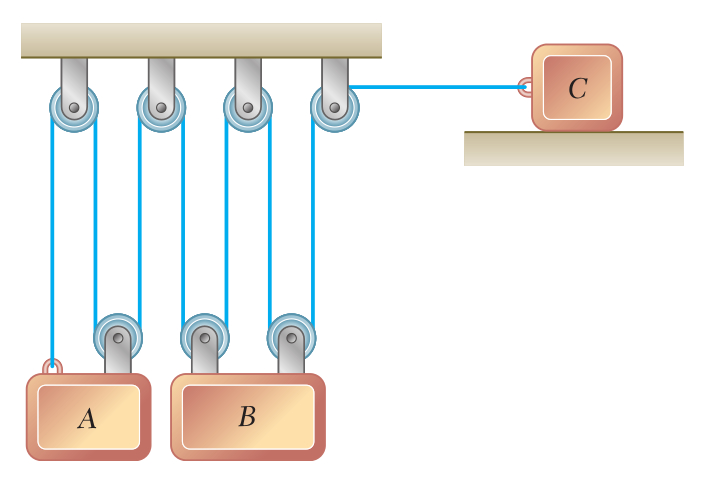
\includegraphics[width=0.5\textwidth]{problema-1.jpg}
\end{figure}

\emph{Soluci\'on:} Como de costumbre, para los bloques $A$ y $B$ definimos el origen en el techo y la direcci\'on positiva hacia abajo, y para el bloque $C$ definimos el origen el cualquier punto al izquierda del bloque y la direcci\'on positiva hacia la derecha. En este caso la ecuaci\'on de ligadura es: 
\begin{align*}
& \ell \; = \; 3 \, x_A(t) + 4 \, x_B(t) + x_C(t) \\
& \Longrightarrow \; 3 \, v_A(t) + 4 v_B(t) + v_C(t) \; = \; 0 \\
& \Longrightarrow \; 3 \, a_A(t) + 4 a_B(t) + a_C(t) \; = \; 0
\end{align*}
Dado que $v_A(0) = -0.030$ m/s y $v_B(0) = +0.020$ m/s tenemos: 
\[
v_C(0) \; = \; -3 \, v_A(0) - 4 \, v_B(0)
\; = \; +0.010 \; \text{m/s} \; = \; +10 \; \text{mm/s}
\]
Adem\'as, como para todo $t \geq 0$ es el caso que $a_A(t)$ es constante y $a_B(t)$ es cero, concluimos que $a_C(t)$ tambi\'en es constante. Para hallar su aceleraci\'on reconocemos que ese cuerpo se encuentra en movimiento rectil\'ineo uniformemente acelerado, \iec
\[
\Delta x_C(t) \; = \; v_C(0) \, t + (1/2) \, a_C \, t^2 
\]
Cuando $t = 3$ s tenemos $\Delta x_C(t) = 0.057$ m. Por lo tanto: 
\[
a_C \; = \;
\frac{2 \, ( \, \Delta x_C(t) - v_C(0) \, t \, )}{t^2} \; = \;
0.006 \; \text{m/s\tsup{2}} \; \equiv \; 6 \; \text{mm/s\tsup{2}}
\]
Finalmente, de la ecuaci\'on de ligadura obtenemos: 
\[
a_A \; = \; -(1/3) \, a_C \; = \; -2 \; \text{m/s\tsup{2}} \; \equiv \; -2 \; \text{mm/s\tsup{2}}
\]

\end{problem}
\fullskip

% =============================================
\begin{problem}
\textbf{[4 Puntos]} Una puerta levadiza se gu\'ia mediante dos ruedas en $A$ y $B$ que giran sobre las correderas horizontal y vertical que se muestran en la figura. Si cuando $\theta = 40\deg$ la velocidad de la rueda $B$ es de 1.5 ft/s hacia arriba, determine \textit{(i)} la velocidad angular de la puerta y \textit{(ii)} la velocidad del extremo $D$ de la puerta. 

\begin{figure}[H]
\centering
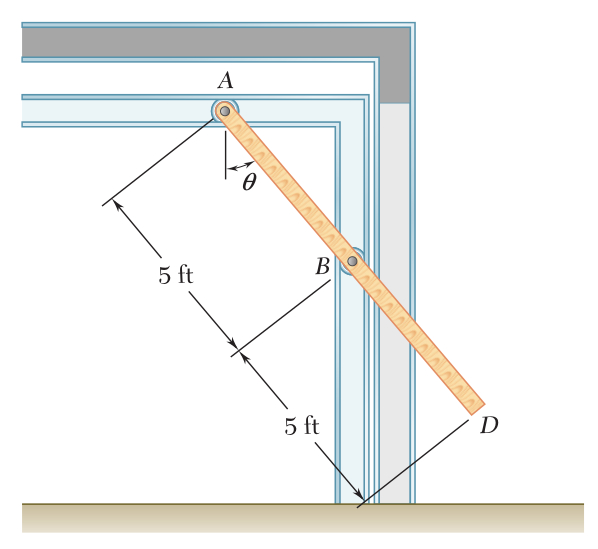
\includegraphics[width=0.5\textwidth]{problema-2.jpg}
\end{figure}

\emph{Soluci\'on:} Primero reconocemos que: 
\begin{align*}
\vec{v_A} \; & = \; ( \, -v_A, 0 \, ) \; \text{ft/s} \\
\vec{v_B} \; & = \; ( \, 0, +1.5 \, ) \; \text{ft/s}
\end{align*}
Adem\'as: 
\begin{align*}
\vec{\hat{r}_{BA}} \; & = \;
( \, -\cos(50\deg), \, +\sin(50\deg) \, ) \; = \;
( \, -0.643, \, +0.766 \, ) \\
\vec{r_{BA}} \; & = \; 5 \, \vec{\hat{r}_{BA}} \; = \;
( \, -3.214, \, +3.830 \, ) \; \text{ft} \\
\vec{r_{BD}} \; & = \; -\vec{r_{BA}} \; = \; 
( \, +3.214, \, -3.830 \, ) \; \text{ft} \\
\end{align*}
Entonces, de la relaci\'on entre las velocidades de $A$ y $B$ obtenemos: 
\begin{align*}
& \vec{v_A} \; = \; \vec{v_B} + \vec{\omega} \times \vec{r_{BA}} \\[1ex]
& \Longrightarrow \; \left[ \begin{array}{c}
-v_A \\ 0
\end{array} \right] \; = \;
\left[ \begin{array}{c}
0 \\ +1.5
\end{array} \right] + 
\left[ \begin{array}{c}
-3.830 \, \omega \\ -3.214 \, \omega
\end{array} \right] \\[1ex]
& \Longrightarrow \; \vec{\omega} \; = \; +0.4667 \, \vec{\hat{k}} \; \text{rad/s}
\end{align*}
Finalmente, calculamos la velocidad en $D$ considerando la velocidad en $B$ :
\begin{align*}
& \vec{v_D} \; = \; \vec{v_B} + \vec{\omega} \times \vec{r_{BD}} \\[1ex]
& \Longrightarrow \; \left[ \begin{array}{c}
+(v_D)_x \\ +(v_D)_y
\end{array} \right] \; = \;
\left[ \begin{array}{c}
0 \\ +1.5
\end{array} \right] + 
\left[ \begin{array}{c}
(+3.830)(0.4667) \\ (+3.214)(0.4667)
\end{array} \right] \\[1ex]
& \Longrightarrow \; \vec{v_B} \; = \; 
\left[ \begin{array}{c}
+1.788 \\ +3.000
\end{array} \right] \, \text{m/s}
\end{align*}

\end{problem}
\fullskip

\end{document}